\documentclass[11pt]{article}

\usepackage{setspace}
\usepackage[margin=1in]{geometry}

% Make table of contents look better
\usepackage{tabularx}
\usepackage{tocloft}
\renewcommand{\cftsecleader}{\cftdotfill{\cftdotsep}}

\usepackage{graphicx}
\usepackage{pdfpages}
\usepackage{hyperref}

% \usepackage[ngerman]{babel}
% \usepackage[T1]{fontenc}
% \usepackage[ansinew]{inputenc}
% \usepackage{lmodern}

% Times New Roman font
\usepackage{txfonts}

\begin{document}

\setlength{\parindent}{2em}

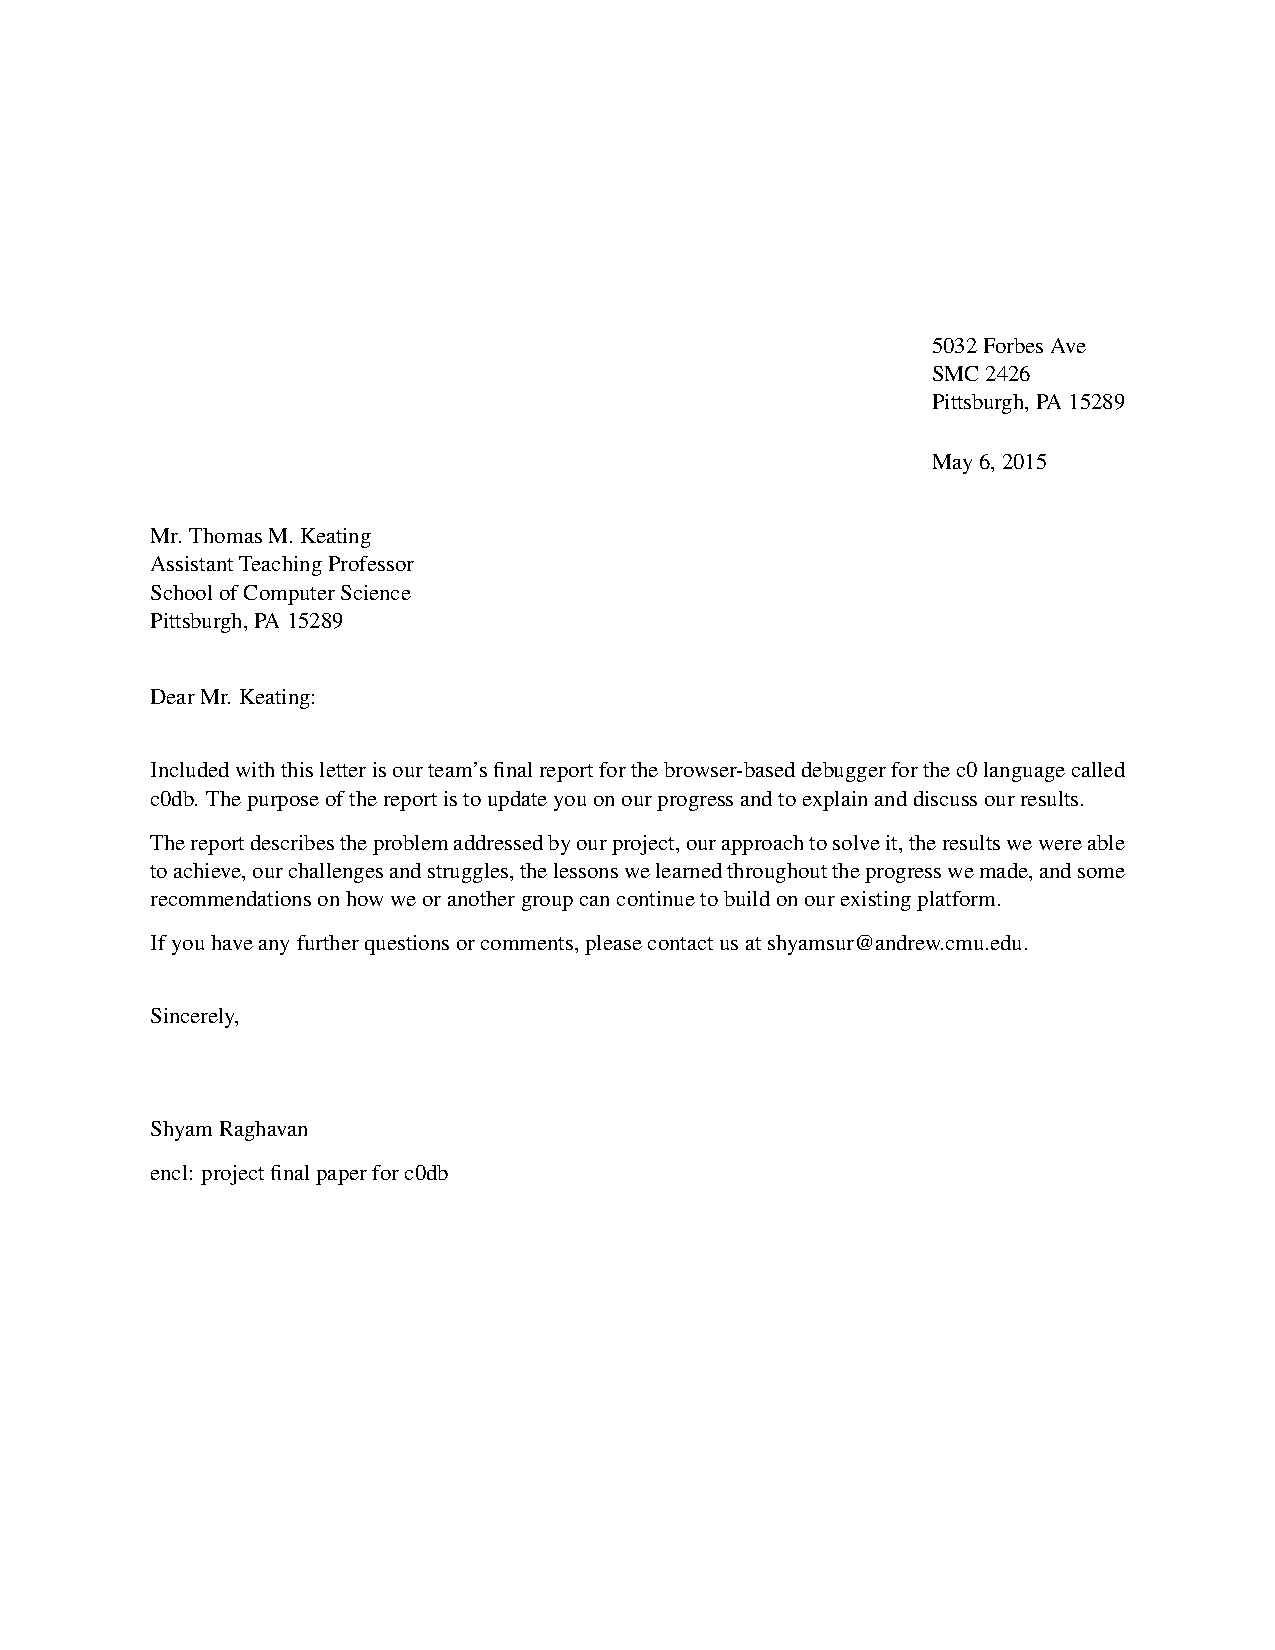
\includepdf[pages={1}]{letter.pdf}

\begin{titlepage}
\clearpage
\thispagestyle{empty}

\begin{center}
{\Huge Final Report}\\
\vspace{10 mm}
{\Huge {\tt c0db}\\[.4em]
The {\tt C0} Debugger}\\
\vspace{10 mm}

Submitted to\\
Mr. Thomas M. Keating\\
Assistant Teaching Professor\\
School of Computer Science\\
Carnegie Mellon University\\
Pittsbugh, PA 15289

\vspace{10 mm}

Prepared by:\\
{\bf Aaron Gutierrez}\\
{\bf Shyam Raghavan}\\
Mitchell Plamann\\
Suhaas Reddy

\vspace{10 mm}

School of Computer Science\\
Carnegie Mellon University\\
\today

\vspace{10 mm}

{\bf Abstract}
\end{center}
\par
Finding problems in code is a difficult and time consuming task, one especially
difficult for programmers learning a new language. To help students more quickly
find bugs and understand how their programs run, we created an online debugger
for the {\tt C0} programming language. The {\tt C0} debugger, {\tt c0db},
enables users to run programs in their browser and break apart the execution
when they don't run correctly.
\end{titlepage}

\pagenumbering{roman}
\tableofcontents
\newpage

\pagenumbering{arabic}

\section{Introduction}

\section{Approach}

\section{Results}
\par
We originally aimed to evaluate our performance against user feedback from both
current and past students. However, due to setbacks in the early stages of
development we were unable to receive significant use feedback from students.
That said, we were able to gather feedback and support from current 15-122
course staff.

In terms of our original vision, {\tt c0db} includes almost every feature we
planned to implement. Users can input code and either run the program straight
through or step through execution instruction by instruction. The only
significant feature that is not currently implemented completely is breakpoints.
Implementing breakpoints turned out to be significantly more difficult than we
anticipated, and given our limited time frame, we were unable to come up with an
adequate solution. We are currently working with Rob Simmons, 15-122 instructor
and maintainer for the {\tt C0} language standard, to extend the language to
support breakpoints more easily going forward.

\begin{figure}[h]
  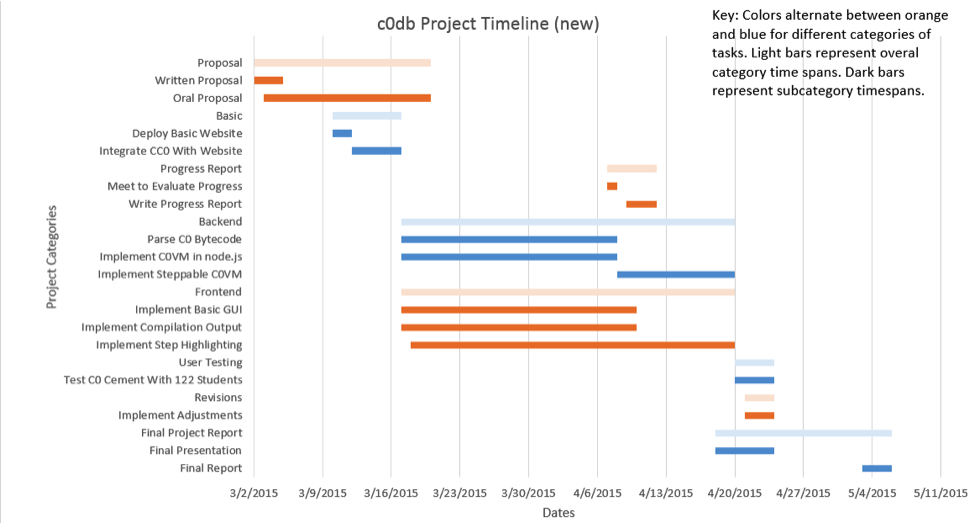
\includegraphics[width=\linewidth]{new-gantt}
  \caption{Revised project Gantt chart}
  \label{gantt}
\end{figure}
Relative to our revised Gantt Chart (Figure \ref{gantt}) we hit every milestone
on time. Both the front-end and back-end teams completed their tasks by the end
of April, at which point we transitioned everyone to user testing, revisions,
and polishing. Both teams were able to recover from the lag reported in our
progress report to complete {\tt c0db}.

\section{Discussion}
\subsection{Reflection}
Our team learned several useful skills while working on this project, ranging
from technical tricks to communication insights. For several of us, this project
represents the most collaboration on a single code base. We effectively employed
the git version control system to manage our code to lesson the work needed to
integrate each person's features. Additionally, several members of our team had
never worked with node.js or JavaScript extensively before this project.
Everyone quickly picked up the new framework and started producing useful
output.

We did face some issues communicating early on, but fortunately we were able to
learn from our problems. Communicating strictly online was not sufficient and
resulted in a lack of ownership and drive that put us behind schedule early on.
We overcame our communication problems by holding brief but regular meetings
face to face to cover what has been accomplished and what tasks come next.

\subsection{Future}
{\tt C0db} is most of what we imagined, but not all. Our overall goal, to make a
tool useful for 15-122 students, may be realized in the fall, but we have more
work to ensure that we present them with the best tool possible. Before the next
semester starts we aim to complete the remaining features we originally planned
to implement: source-level breakpoints, multi-file support, and a refined
interface. If we can implement these three features, {\tt c0db} could see proper
adoption by 15-122 in the fall, where it would be used by over 300 students from
across Carnegie Mellon. If {\tt c0db} is adopted by 15-122, we would truly have
achieved the goal for our project: create a tool to better the CMU community.

\section{Sources Cited}

\end{document}
